% Font options: 10pm, 11pt, 12pt
% Align headings left instead of center: nocenter
\documentclass[xcolor=x11names,compress]{beamer}\usepackage[]{graphicx}\usepackage[]{color}
%% maxwidth is the original width if it is less than linewidth
%% otherwise use linewidth (to make sure the graphics do not exceed the margin)
\makeatletter
\def\maxwidth{ %
  \ifdim\Gin@nat@width>\linewidth
    \linewidth
  \else
    \Gin@nat@width
  \fi
}
\makeatother

\definecolor{fgcolor}{rgb}{0.345, 0.345, 0.345}
\newcommand{\hlnum}[1]{\textcolor[rgb]{0.686,0.059,0.569}{#1}}%
\newcommand{\hlstr}[1]{\textcolor[rgb]{0.192,0.494,0.8}{#1}}%
\newcommand{\hlcom}[1]{\textcolor[rgb]{0.678,0.584,0.686}{\textit{#1}}}%
\newcommand{\hlopt}[1]{\textcolor[rgb]{0,0,0}{#1}}%
\newcommand{\hlstd}[1]{\textcolor[rgb]{0.345,0.345,0.345}{#1}}%
\newcommand{\hlkwa}[1]{\textcolor[rgb]{0.161,0.373,0.58}{\textbf{#1}}}%
\newcommand{\hlkwb}[1]{\textcolor[rgb]{0.69,0.353,0.396}{#1}}%
\newcommand{\hlkwc}[1]{\textcolor[rgb]{0.333,0.667,0.333}{#1}}%
\newcommand{\hlkwd}[1]{\textcolor[rgb]{0.737,0.353,0.396}{\textbf{#1}}}%
\let\hlipl\hlkwb

\usepackage{framed}
\makeatletter
\newenvironment{kframe}{%
 \def\at@end@of@kframe{}%
 \ifinner\ifhmode%
  \def\at@end@of@kframe{\end{minipage}}%
  \begin{minipage}{\columnwidth}%
 \fi\fi%
 \def\FrameCommand##1{\hskip\@totalleftmargin \hskip-\fboxsep
 \colorbox{shadecolor}{##1}\hskip-\fboxsep
     % There is no \\@totalrightmargin, so:
     \hskip-\linewidth \hskip-\@totalleftmargin \hskip\columnwidth}%
 \MakeFramed {\advance\hsize-\width
   \@totalleftmargin\z@ \linewidth\hsize
   \@setminipage}}%
 {\par\unskip\endMakeFramed%
 \at@end@of@kframe}
\makeatother

\definecolor{shadecolor}{rgb}{.97, .97, .97}
\definecolor{messagecolor}{rgb}{0, 0, 0}
\definecolor{warningcolor}{rgb}{1, 0, 1}
\definecolor{errorcolor}{rgb}{1, 0, 0}
\newenvironment{knitrout}{}{} % an empty environment to be redefined in TeX

\usepackage{alltt}
%\documentclass[xcolor=x11names,compress,handout]{beamer}
\usepackage[]{graphicx}
\usepackage[]{color}
\usepackage{booktabs}
\usepackage{hyperref}
\usepackage{tikz}
\usepackage{multirow}
\usepackage{multicol}
\usepackage{dcolumn}
\usepackage{bigstrut}
\usepackage{amsmath} 
\usepackage{xcolor,colortbl}
\usepackage{amssymb}
%\newcommand{\done}{\cellcolor{teal}#1}

%% Beamer Layout %%%%%%%%%%%%%%%%%%%%%%%%%%%%%%%%%%
\useoutertheme[subsection=false,shadow]{miniframes}
\useinnertheme{default}
\usefonttheme{serif}
\usepackage{Arev}
\usepackage{pdfpages}

\setbeamerfont{title like}{shape=\scshape}
\setbeamerfont{frametitle}{shape=\scshape, size=\normalsize}

\definecolor{dkblue}{RGB}{0,0,102}

\setbeamercolor*{lower separation line head}{bg=dkblue} 
\setbeamercolor*{normal text}{fg=black,bg=white} 
\setbeamercolor*{alerted text}{fg=red} 
\setbeamercolor*{example text}{fg=black} 
\setbeamercolor*{structure}{fg=black} 
 
\setbeamercolor*{palette tertiary}{fg=black,bg=black!10} 
\setbeamercolor*{palette quaternary}{fg=black,bg=black!10} 

\renewcommand{\(}{\begin{columns}}
\renewcommand{\)}{\end{columns}}
\newcommand{\<}[1]{\begin{column}{#1}}
\renewcommand{\>}{\end{column}}

\setbeamertemplate{navigation symbols}{} 
\setbeamertemplate{footline}[frame number]
\setbeamertemplate{caption}{\raggedright\insertcaption\par}

\setbeamersize{text margin left=5pt,text margin right=5pt}

\AtBeginSection{\frame{\sectionpage}}
\usepackage{xcolor}
\hypersetup{
    colorlinks,
    linkcolor={red!50!black},
    citecolor={blue!50!black},
    urlcolor={blue!80!black}
}

%%%%%%%%%%%%%%%%%%%%%%%%%%%%%%%%%%%%%%%%%%%%%%%%%%




\title{FLS 6441 - Methods III: Explanation and Causation}
\subtitle{Week 1 - Review}
\author{Jonathan Phillips}
\date{February 2019}
\IfFileExists{upquote.sty}{\usepackage{upquote}}{}
\begin{document}

\frame{\titlepage}

\begin{frame}
\frametitle{Probability Review}
\begin{center}
$Pr(A)=\frac{\text{Number of times A occurs}}{\text{Number of Trials}}$ \\
Joint Probability: $Pr(A \cap B) = P(A,B)$ \\
Conditional Probability: $Pr(A|B) = \frac{Pr(A \cap B)}{Pr(B)}$ \\
\end{center}
\end{frame}

\begin{frame}
\frametitle{Probability Review}
\begin{center}
Independence: $A$ and $B$ are independent iff $Pr(A \cap B) = Pr(A) * Pr(B)$ \\
Then: $Pr(A|B) = \frac{Pr(A \cap B)}{Pr(B)} = \frac{Pr(A) * Pr(B)}{Pr(B)} = Pr(A)$ \\
\end{center}
\end{frame}

\begin{frame}
\frametitle{Probability Review}
\begin{itemize}
\item A = It's raining in Osasco right now
\item B = I flip this coin and get Heads
\item Are these events independent?
\pause
\item Yes! One does not affect the other at all
\item So $Pr(A \cap B) = Pr(A)*Pr(B)$
\item $Pr(A \cap B) = 0.3 * 0.5 = 0.15$
\end{itemize}
\end{frame}

\begin{frame}
\frametitle{Probability Review}
\begin{itemize}
\item A = It's raining in Osasco right now
\item B = It's raining in S\~{a}o Paulo right now
\item Are these events independent?
\pause
\item No! If you know it's raining in Osasco there's a stronger chance it will be raining in S\~{a}o Paulo
\item So $Pr(A \cap B) \neq Pr(A)*Pr(B)$
\item $Pr(A \cap B) \neq 0.3 * 0.5 = 0.15$
\item $Pr(A \cap B) > 0.15$ (probably)
\end{itemize}
\end{frame}

\begin{frame}
\frametitle{Probability Review}

\begin{multicols}{2}
\begin{knitrout}
\definecolor{shadecolor}{rgb}{0.969, 0.969, 0.969}\color{fgcolor}
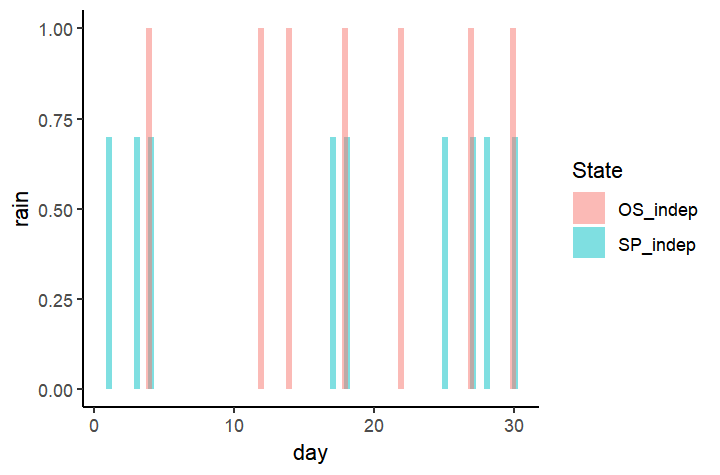
\includegraphics[width=\maxwidth]{figure/rain_graph1-1} 

\end{knitrout}
\footnotesize
$Pr(\text{Rain in Osasco})*Pr(\text{Rain in S\~{a}o Paulo}) = 0.2 * 0.2 = 0.04$ \\
$Pr(\text{Rain in Osasco} \cap  \text{Rain in S\~{a}o Paulo}) = 0.05$ \\
$Pr(\text{Rain in Osasco})*Pr(\text{Rain in S\~{a}o Paulo}) = Pr(\text{Rain in Osasco} \cap  \text{Rain in S\~{a}o Paulo})$ \\
\normalsize

\columnbreak

\begin{knitrout}
\definecolor{shadecolor}{rgb}{0.969, 0.969, 0.969}\color{fgcolor}
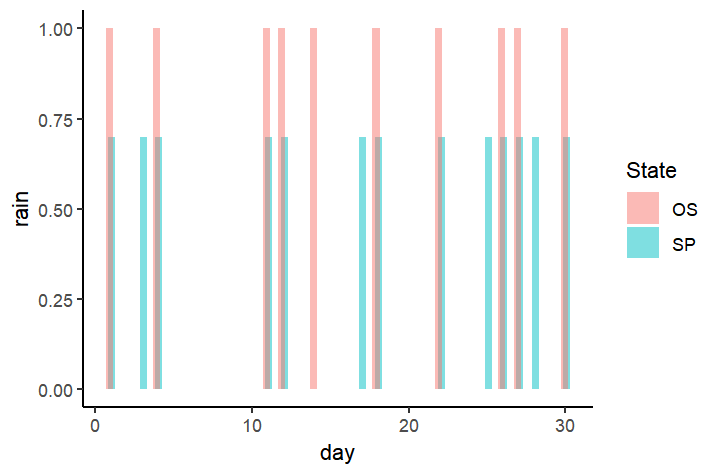
\includegraphics[width=\maxwidth]{figure/rain_graph2-1} 

\end{knitrout}
\footnotesize
$Pr(\text{Rain in Osasco})*Pr(\text{Rain in S\~{a}o Paulo}) = 0.37 * 0.36 = 0.13$ \\
$Pr(\text{Rain in Osasco} \cap  \text{Rain in S\~{a}o Paulo}) = 0.25$ \\
$Pr(\text{Rain in Osasco})*Pr(\text{Rain in S\~{a}o Paulo}) \neq Pr(\text{Rain in Osasco} \cap  \text{Rain in S\~{a}o Paulo})$ \\
\normalsize
\end{multicols}
\end{frame}

\section{Explanation}

\begin{frame}
\frametitle{Learning from Data}
\begin{itemize}
\item What does it mean to explain something?
\pause
\item To give an account of what happens, \textit{and why}
\begin{itemize}
\item The 'chain of causation'
\end{itemize}
\end{itemize}
\end{frame}

\setbeamercolor{background canvas}{bg=}
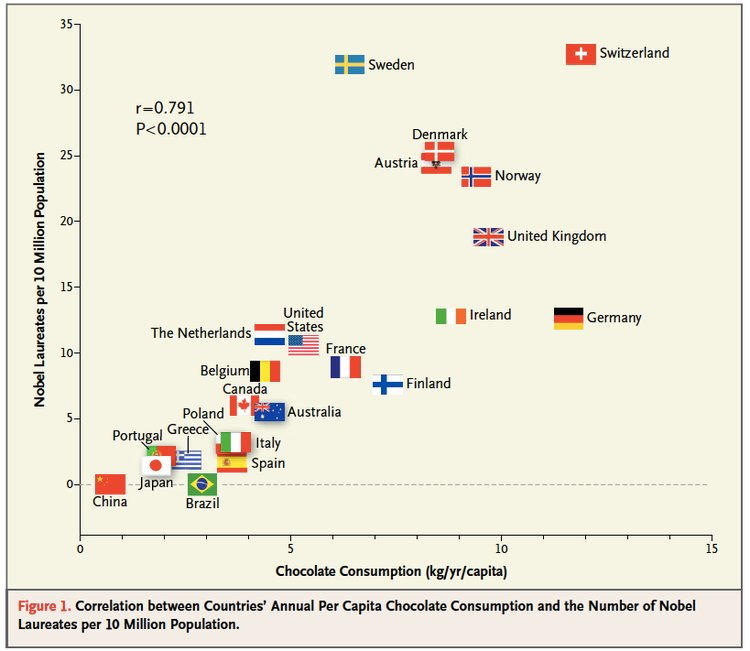
\includegraphics[width=0.9\textwidth]{Chocolate_Nobel.jpg}

\begin{frame}
\frametitle{Learning from Data}
\small
\begin{itemize}
\item Why isn't correlation enough?
\pause
\begin{itemize}
\item For \textbf{prediction}, correlation is fine: If we know a country has chocolate consumption of 10kg/yr/capita we can reasonably predict it will have about 25 Nobel Laureates
\pause
\item But for \textbf{intervention}, correlation does not help: forcing people to eat more chocolate does nothing on its own to produce more Nobel Laureates
\pause
\item For \textbf{explanation}, correlation also fails - it is no \textit{explanation} to say that Switzerland has the most Nobel Laureates because it has the highest chocolate consumption
\end{itemize}
\end{itemize}
\normalsize
\end{frame}

\begin{frame}
\frametitle{Learning from Data}
\begin{itemize}
\item Two perspectives on explanation:
\end{itemize}
\pause
\begin{table}[htbp]
  \centering
    \begin{tabular}{|>{\raggedright}p{5cm}|p{5cm}|}
    \toprule
    \textbf{Causes of Effects} & \textbf{Effects of Causes} \\
    \midrule
    What caused Y? & Does D cause Y? \\
    \midrule
    Why does Switzerland have so many Nobel laureates? & Does chocolate cause more Nobel laureates? \\
    \bottomrule
    \end{tabular}%
  \label{tab:addlabel}%
\end{table}%
\end{frame}

\begin{frame}
\frametitle{Learning from Data}
\begin{itemize}
\item Two perspectives on explanation:
\end{itemize}
\begin{multicols}{2}
\begin{knitrout}
\definecolor{shadecolor}{rgb}{0.969, 0.969, 0.969}\color{fgcolor}
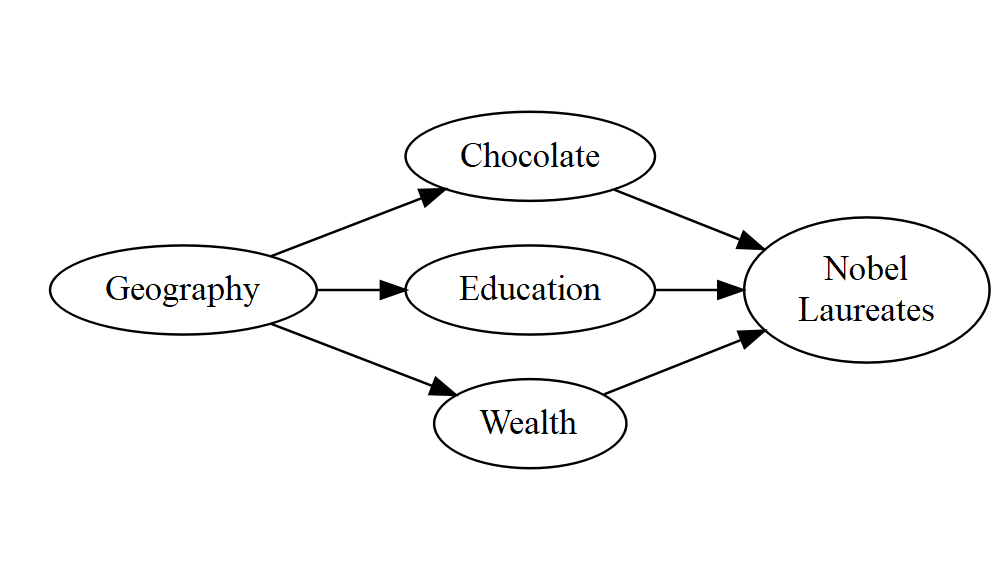
\includegraphics[width=\maxwidth]{figure/explanation1-1} 

\end{knitrout}
\pause
\begin{itemize}
\item Identifying the source of \textbf{ALL} of the variation in Nobel Laureates
\pause
\item An infinite task!
\end{itemize}
\pause
\columnbreak
\begin{knitrout}
\definecolor{shadecolor}{rgb}{0.969, 0.969, 0.969}\color{fgcolor}
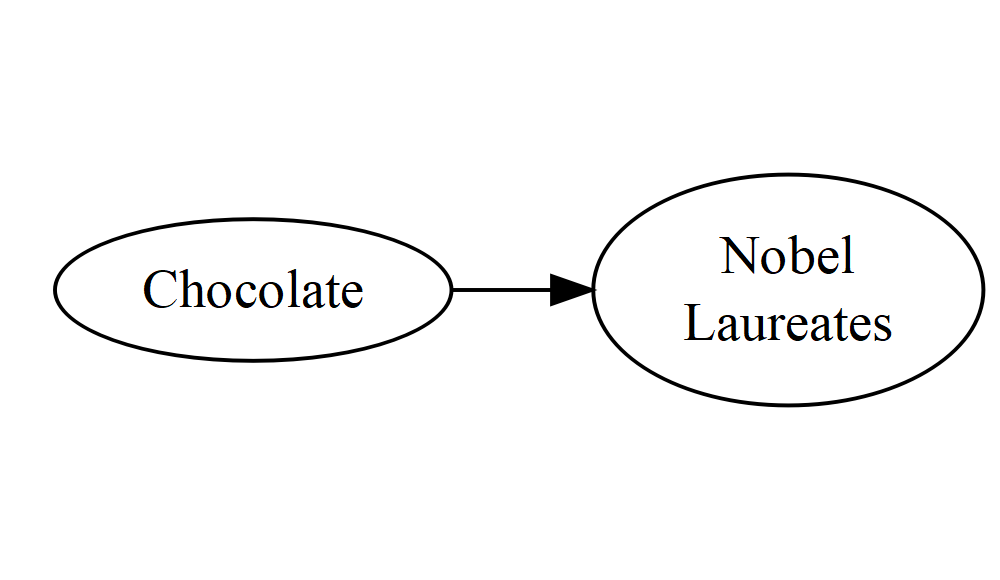
\includegraphics[width=\maxwidth]{figure/explanation2-1} 

\end{knitrout}
\pause
\begin{itemize}
\item Identifying how much \textbf{ONE} variable causes variation in Nobel Laureates
\pause
\item This we can do!
\end{itemize}
\end{multicols}
\end{frame}

\begin{frame}
\frametitle{Explanation}
\begin{itemize}
\item A focus on a single explanatory variable $D$ requires a clear definition of \textbf{'Treatment'}
\item AND to clearly define a \textbf{'Control'}
\begin{itemize}
\item What is the opposite of investing \$1bn in education?
\item No investment, or investing it elsewhere?
\end{itemize}
\item Define treatment:
\end{itemize}
\[D_i = 
\begin{cases}
1 \text{, if treated} \\
0 \text{, if not treated}
\end{cases}
\]
\end{frame}

\begin{frame}
\frametitle{Causal Inference}
\begin{itemize}
\item Defining our outcome:
\begin{itemize}
\item Is it the outcome we really care about? Or just what's easy to measure?
\item Tempting to look at many outcomes, but the risk of 'cherry-picking'
\begin{itemize}
\item All outcomes are \textbf{probabilistic} (due to all the other factors we haven't accounted for)
\item If we study 20 outcomes, on average one will show a significant effect even with no real causal effect
\end{itemize}
\item So we also want a \textbf{single outcome} usually
\end{itemize}
\end{itemize}
\end{frame}

\begin{frame}
\frametitle{Causal Inference}
\begin{itemize}
\item What are the \textbf{units} of our analysis?
\item Countries? Political Parties? Individuals?
\item eg. How does electoral system affect attitudes to redistribution?
\begin{itemize}
\item Treatment at the national level
\item Outcome at the individual level
\item Measurement needed at the lowest (individual) level
\end{itemize}
\item Units are \textbf{time-specific}: the same person 10 minutes later is a different unit
\end{itemize}
\end{frame}

\section{Causal Inference}

\begin{frame}
\frametitle{Causal Inference}
\begin{itemize}
\item Why wasn't regression enough for explanation?
\begin{enumerate}
\item Omitted Variables
\item Reverse Causation
\item Selection Bias
\item Measurement Bias
\item Lack of Overlap
\end{enumerate}
\item In all of these cases the values in our data hid the real causal relationship
\end{itemize}
\end{frame}

\begin{frame}
\frametitle{Causal Inference}
\begin{itemize}
\item Omitted Variables
\end{itemize}
\begin{multicols}{2}
A real causal relationship:
\begin{knitrout}
\definecolor{shadecolor}{rgb}{0.969, 0.969, 0.969}\color{fgcolor}
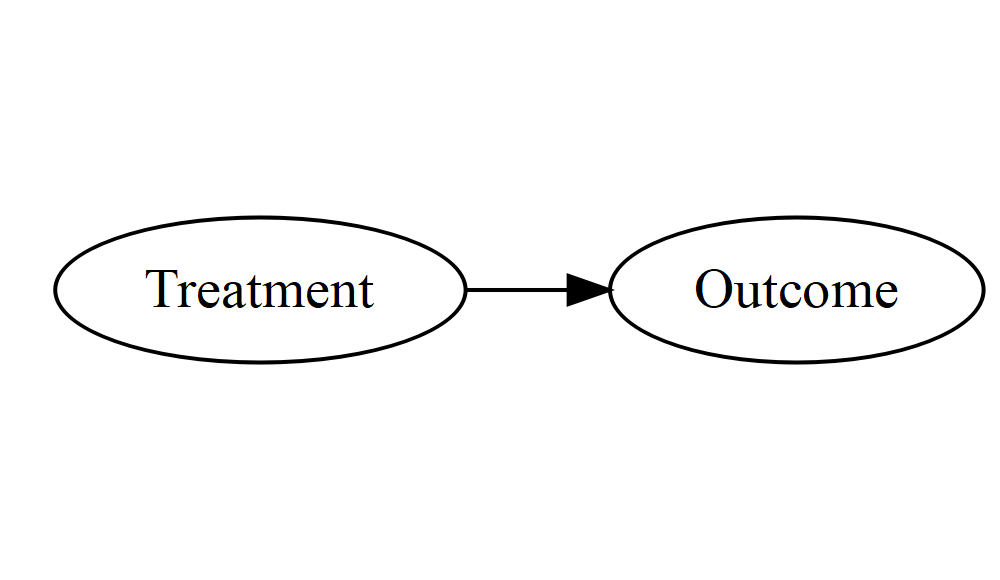
\includegraphics[width=\maxwidth]{figure/explanation3-1} 

\end{knitrout}
\columnbreak
Being misled by omitted variable bias:
\begin{knitrout}
\definecolor{shadecolor}{rgb}{0.969, 0.969, 0.969}\color{fgcolor}
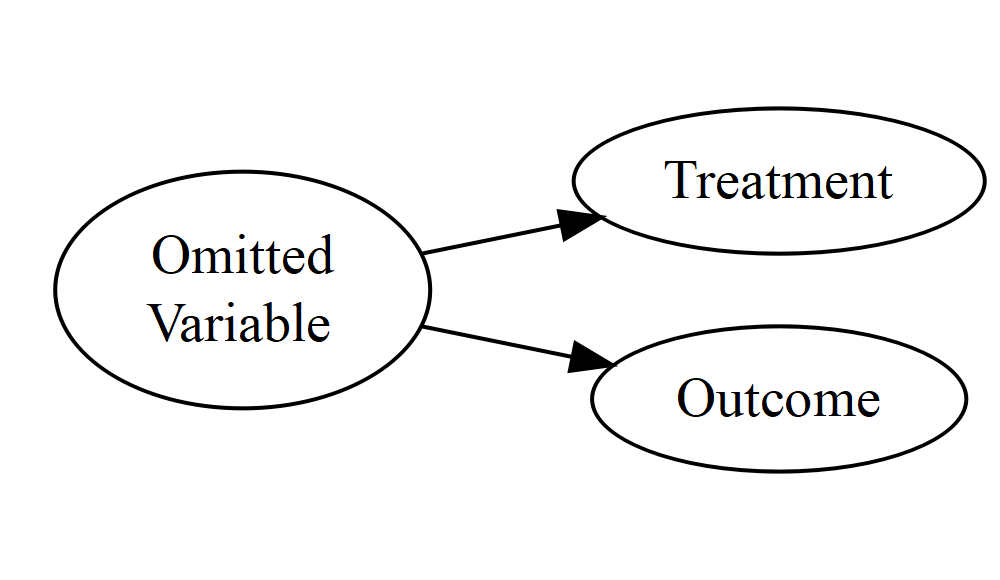
\includegraphics[width=\maxwidth]{figure/explanation4-1} 

\end{knitrout}
\end{multicols}
\end{frame}

\begin{frame}
\frametitle{Causal Inference}
\begin{itemize}
\item Reverse Causation
\end{itemize}
\begin{multicols}{2}
A real causal relationship:
\begin{knitrout}
\definecolor{shadecolor}{rgb}{0.969, 0.969, 0.969}\color{fgcolor}
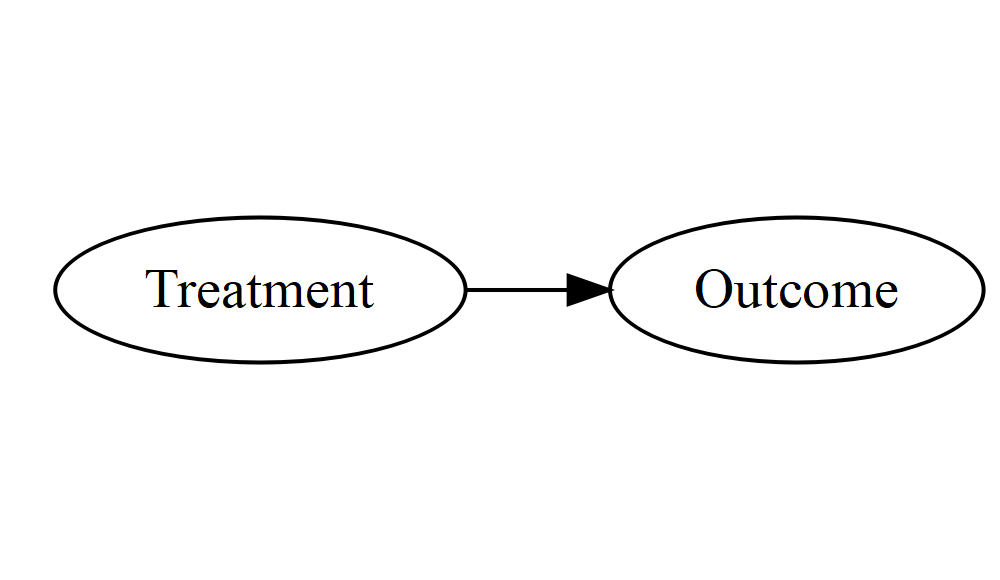
\includegraphics[width=\maxwidth]{figure/explanation5-1} 

\end{knitrout}
\columnbreak
Being misled by reverse causation:
\begin{knitrout}
\definecolor{shadecolor}{rgb}{0.969, 0.969, 0.969}\color{fgcolor}
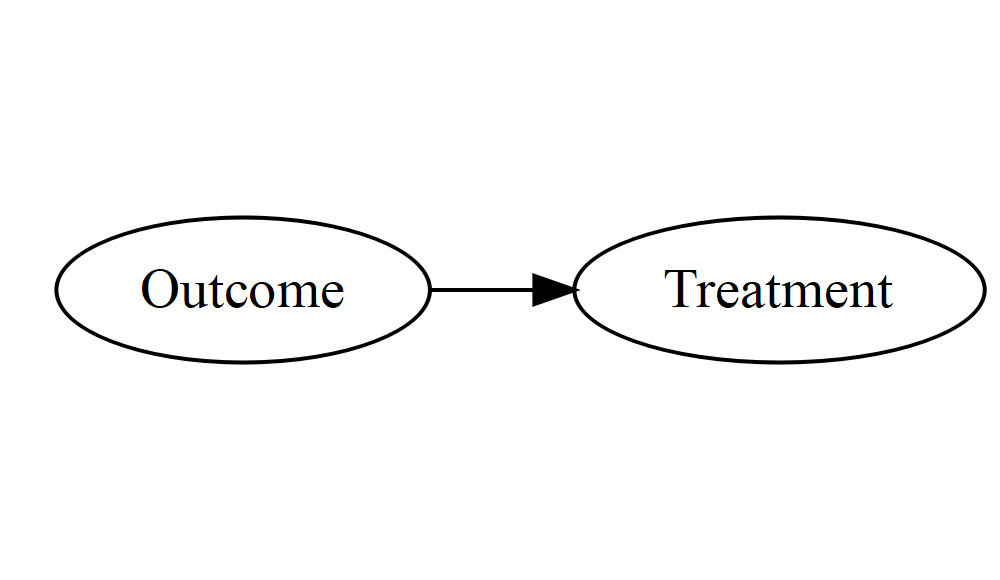
\includegraphics[width=\maxwidth]{figure/explanation6-1} 

\end{knitrout}
\end{multicols}
\end{frame}

\begin{frame}
\frametitle{Causal Inference}
\begin{itemize}
\item Reverse Causation
\end{itemize}
\begin{multicols}{2}
A real causal relationship:
\begin{knitrout}
\definecolor{shadecolor}{rgb}{0.969, 0.969, 0.969}\color{fgcolor}
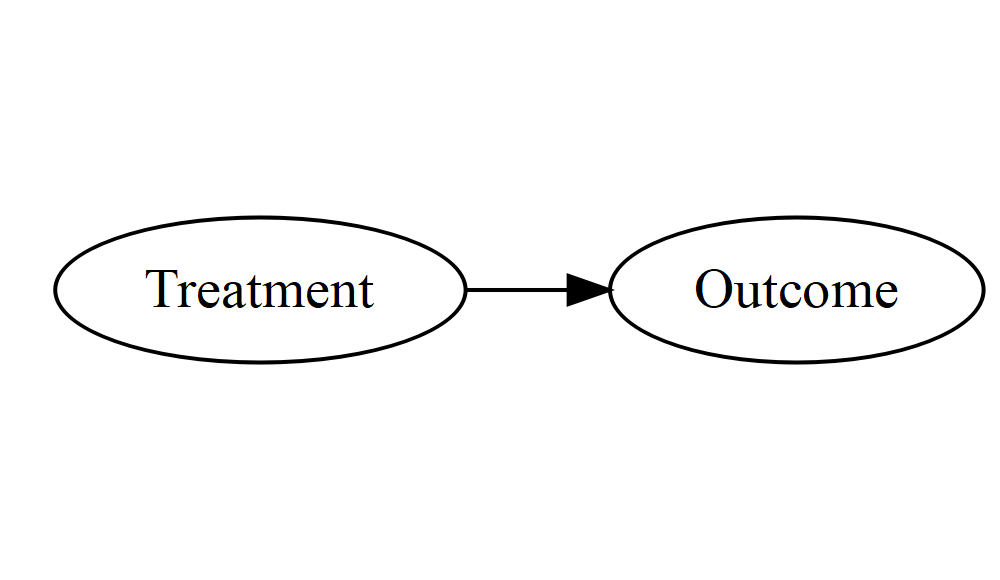
\includegraphics[width=\maxwidth]{figure/explanation7-1} 

\end{knitrout}
\columnbreak
Being misled by Selection Bias:
\begin{knitrout}
\definecolor{shadecolor}{rgb}{0.969, 0.969, 0.969}\color{fgcolor}
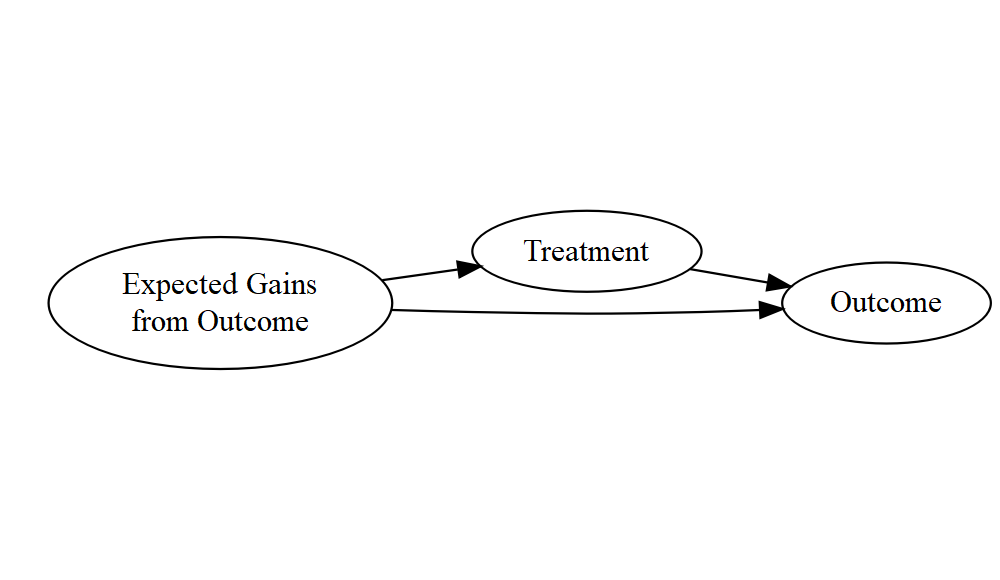
\includegraphics[width=\maxwidth]{figure/explanation8-1} 

\end{knitrout}
\end{multicols}
\end{frame}

\begin{frame}
\frametitle{Causal Inference}
\begin{itemize}
\item In all of these cases, \textbf{which units get 'treated' ($D_i=1$)} affect our estimate of the relationship between $D$ and $Y$
\pause
\begin{itemize}
\item This is the \textbf{Treatment Assignment Mechanism}
\pause
\end{itemize}
\item \textbf{Omitted Variable Bias} - the Swiss consume chocolate because they're in Europe, which also affects production of Nobel Laureates
\pause
\item \textbf{Reverse Causation} - the Swiss consume chocolate \textit{because} they have a lot of Nobel laureates
\pause
\item \textbf{Selection Bias} - the Swiss \textit{choose} to eat a lot of chocolate because they know it will be really effective at producing Nobel Laureates
\pause
\item Messy treatment assignment mechanisms are why basic regression is no use for explanation
\begin{itemize}
\item It means our control cases are really misleading
\item South Africa is our counterfactual for Switzerland
\item What would happen if the 'untreated' units got treated?
\end{itemize}
\end{itemize}
\end{frame}

\begin{frame}
\frametitle{Causal Inference}
\begin{itemize}
\item The \textbf{causal effect} of treatment is how each unit's outcome differs when it is treated and not treated
\pause
\item This means comparing the \textbf{Potential Outcomes} for unit $i$:
\[
Y_{Di} = 
\begin{cases}
Y_{1i}\text{   Potential Outcome if unit i treated} \\
Y_{0i}\text{   Potential Outcome if unit i NOT treated}
\end{cases}
\]
\item Individual Treatment Effect for unit $i$ $ = Y_{1i} - Y_{0i}$
\end{itemize}
\end{frame}

\begin{frame}
\frametitle{Causal Inference}
\begin{itemize}
\item The \textbf{causal effect} of treatment is how each unit's outcome differs when it is treated and not treated
\pause
\item This means comparing the \textbf{Potential Outcomes} for unit $i$:
\[
Y_{Di} = 
\begin{cases}
Y_{1i}\text{   GDP Growth of Brazil in 2010 if a Democracy} \\
Y_{0i}\text{   GDP Growth of Brazil in 2010 if NOT a Democracy}
\end{cases}
\]
\item Individual Treatment Effect for unit $i$ $ = Y_{1i} - Y_{0i}$
\end{itemize}
\end{frame}

\begin{frame}
\frametitle{Causal Inference}
\begin{itemize}
\item We are relying on \textbf{counterfactuals}
\pause
\begin{itemize}
\item What would have happened to the same unit if the treatment had not happened?
\pause
\item Would World War I still have happened if Archduke Franz Ferdinand had not been assassinated in 1914?
\pause
\item Would Brazil have won the 2014 World Cup if Neymar had not been injured?
\pause
\end{itemize}
\end{itemize}
\end{frame}


\begin{frame}
\frametitle{Causal Inference}
\footnotesize
\begin{table}[htbp]
  \centering
  \caption{Potential Outcomes are just another Variable}
    \begin{tabular}{|p{2.4cm}|p{2.4cm}|p{2.4cm}|r|}
    \hline
          & \multicolumn{1}{p{2.4cm}|}{GDP Growth if Democracy} & \multicolumn{1}{p{2.4cm}|}{GDP Growth if  NOT Democracy} &  \bigstrut\\
    \hline
          & \multicolumn{1}{l|}{$Y_1$} & \multicolumn{1}{l|}{$Y_0$} & \multicolumn{1}{l|}{Treatment Effect} \bigstrut\\
    \hline
    Brasil & 4     & 2     & 2 \bigstrut\\
    \hline
    Argentina & 7    & 3     & 4 \bigstrut\\
    \hline
    Bolivia & 2     & 4     & -2 \bigstrut\\
    \hline
    Colombia & 11    & 11    & 0 \bigstrut\\
    \hline
    Peru & 6     & 2     & 4 \bigstrut\\
    \hline
    \end{tabular}%
  \label{tab:addlabel}%
\end{table}%
\normalsize
\end{frame}

\begin{frame}
\frametitle{Causal Inference}
\begin{itemize}
\item Political Science is not about explaining individual events
\pause
\item We ideally want general theories that apply to many situations
\pause
\item To explain a systematic treatment - not a single event - we need \textbf{multiple counterfactual comparisons}
\pause
\item We know how democracy works in Europe; the question is what will happen if it becomes more common in Africa?
\pause
\item We want to calculate an \textbf{Average Treatment Effect} 
\pause 
\item $ATE= \frac{\sum_i (Y_{1i} - Y_{0i})}{N}$
\end{itemize}
\end{frame}

\begin{frame}
\frametitle{Causal Inference}
\footnotesize
\begin{table}[htbp]
  \centering
  \caption{Potential Outcomes are just another Variable}
    \begin{tabular}{|p{2.4cm}|p{2.4cm}|p{2.4cm}|r|}
    \hline
          & \multicolumn{1}{p{2.4cm}|}{GDP Growth if Democracy} & \multicolumn{1}{p{2.4cm}|}{GDP Growth if  NOT Democracy} &  \bigstrut\\
    \hline
          & \multicolumn{1}{p{2.4cm}|}{$Y_1$} & \multicolumn{1}{l|}{$Y_0$} & \multicolumn{1}{l|}{Treatment Effect} \bigstrut\\
    \hline
    Brasil & 4     & 2     & 2 \bigstrut\\
    \hline
    Argentina & 7    & 3     & 4 \bigstrut\\
    \hline
    Bolivia & 2     & 4     & -2 \bigstrut\\
    \hline
    Colombia & 7    & 7    & 0 \bigstrut\\
    \hline
    Peru & 5     & 4     & 1 \bigstrut\\
    \hline
    \textbf{Average Treatment Effect} & \textbf{5} & \textbf{4} & \textbf{1} \bigstrut\\
    \hline
    \end{tabular}%
  \label{tab:addlabel}%
\end{table}%
\normalsize
\end{frame}

%Messy - tidy up below
\begin{frame}
\frametitle{Causal Inference}
\begin{itemize}
\item \textbf{The Fundamental Problem of Causal Inference}
\begin{itemize}
\item No units can receive \textbf{both} treatment and control
\item So we can never observe both $Y_1$ and $Y_0$ for the same unit
\end{itemize}
\end{itemize}
\end{frame}

\begin{frame}
\frametitle{Causal Inference}
\footnotesize
\begin{table}[htbp]
  \centering
  \caption{Potential Outcomes Example}
    \begin{tabular}{|p{1.8cm}|p{2.2cm}|p{2.2cm}|p{1.8cm}|r|}
    \hline
          & \multicolumn{1}{p{1.8cm}|}{PR System?} & \multicolumn{1}{p{2.2cm}|}{Investment in Education if PR system} & \multicolumn{1}{p{2.2cm}|}{Investment in Education if FPTP system} &  \bigstrut\\
    \hline
          & \multicolumn{1}{p{1.8cm}|}{$D_i$} & \multicolumn{1}{p{2.2cm}|}{$Y_1$} & \multicolumn{1}{p{2.2cm}|}{$Y_0$} & \multicolumn{1}{p{1.8cm}|}{Treatment Effect} \bigstrut\\
    \hline
    Brasil & 1 & 8     & ?      & ? \bigstrut\\
    \hline
    Argentina & 1 & 10    & ?      & ? \bigstrut\\
    \hline
    Bolivia & 0 & ?     & 4     & ? \bigstrut\\
    \hline
    Colombia & 0 &  ?   & 11    & ? \bigstrut\\
    \hline
    Peru & 0 & ?     & 2     & ? \bigstrut\\
    \hline
    \end{tabular}%
  \label{tab:addlabel}%
\end{table}%
\normalsize
\end{frame}

\begin{frame}
\frametitle{Causal Inference}
\begin{itemize}
\item We can't even look at the change in countries that switch to a PR system
\begin{itemize}
\item What if \textbf{all} countries had started to invest more in education at the same time, for different reasons?
\item The potential outcome for Country X in time 1 is different to at time 2
\end{itemize}
\item So we need to consider the \textbf{counterfactual} - what would have happened if the country had \textbf{not} switched to a PR system?
\item So we can only estimate the effect by comparing \textbf{across} units
\item That is why we are doing causal \textbf{inference}, not causal proof
\end{itemize}
\end{frame}

\begin{frame}
\frametitle{Causal Inference}
\begin{itemize}
\item So we need to consider the exact \textbf{counterfactual} - what would have happened if the country had \textbf{not} switched to a PR system?
\pause
\begin{itemize}
\item This is \textbf{impossible} to know
\pause
\item We can only \textit{estimate} the effect by comparing \textbf{across} units in some way
\pause
\item That is why we are doing causal \textbf{inference}, not causal proof
\end{itemize}
\end{itemize}
\end{frame}

\begin{frame}
\frametitle{Causal Inference}
\begin{itemize}
\item To compare across units we need counterfactuals: \textbf{control} units that do not receive treatment
\item Control units can never be perfect substitutes
\item Causal Inference is all about identifying a \textbf{plausible counterfactual}
\begin{itemize}
\item Plausible means that the potential outcomes of the control unit are the same as those of the treated unit
\end{itemize}
\end{itemize}
\end{frame}

\begin{frame}
\frametitle{Causal Inference}
\begin{itemize}
\item The comparability of treatment and control units depends on how they got to be treated
\begin{itemize}
\item On the \textbf{treatement assignment mechanism}
\end{itemize}
\item If we 'treated' an outlier like B\'{u}zios in Rio, could we find a comparable control unit?
\item Comparisons are easier where the \textbf{treatment assignment mechanism is independent of potential outcomes}
\begin{itemize}
\item This makes it more likely that potential outcomes are 'balanced' and comparable
\end{itemize}
\end{itemize}
\end{frame}

\section{Rest of the Course}

\begin{frame}
\frametitle{Causal Inference}
\begin{itemize}
\item The rest of the course is mostly about the types of treatment assignment mechanisms that \textbf{avoid these biases} and provide plausible counterfactuals
\end{itemize}
\end{frame}

\begin{frame}
\frametitle{Causal Inference}
\begin{enumerate}
\item \textbf{Controlled Experiments} where we \textbf{control} the treatment assignment
\begin{itemize}
\item Field Experiments
\item Survey Experiments
\item Lab Experiments
\end{itemize}
\end{enumerate}
\end{frame}

\begin{frame}
\frametitle{Causal Inference}
\begin{enumerate}
 \setcounter{enumi}{1}
\item \textbf{Natural Experiments} where the assignment mechanism creates balanced potential outcomes
\begin{itemize}
\item Randomized natural experiments
\item Regression Discontinuities
\item Instrumental Variables
\end{itemize}
\end{enumerate}
\end{frame}

\begin{frame}
\frametitle{Causal Inference}
\begin{enumerate}
\setcounter{enumi}{2}
\item \textbf{Observable Studies:} What if no suitable treatment assignments are available?
\begin{itemize}
\item No historical examples of natural experiments
\item Not feasible or ethical to run a field experiment
\end{itemize}
\end{enumerate}
\begin{itemize}
\item Remember the purpose of using these specific treatment assignment mechanisms is to achieve \textbf{comparable potential outcomes}
\item One alternative way of making potential outcomes comparable is to \textbf{selectively use Observable Data}
\begin{itemize}
\item Difference-in-Differences
\item Controlling for confouding variables
\item Matching
\end{itemize}
\end{itemize}
\end{frame}

\begin{frame}
\frametitle{Causal Inference}
\begin{table}[htbp]
  \centering
  \caption{Analysis Types and Assumptions}
    \resizebox*{1.1\textheight}{!}{\begin{tabular}{|r|l|p{2.5cm}|p{2.5cm}|p{2.5cm}|p{6cm}|}
    \hline
    \multicolumn{1}{|r|}{\textbf{Week}} & \multicolumn{1}{l|}{\textbf{Assumption:
}} & \textbf{Researcher Controls Treatment Assignment?} & \textbf{Treatment Assignment Independent of Potential Outcomes} & \textbf{SUTVA} & \multicolumn{1}{p{2cm}|}{\textbf{Additional Assumptions}} \bigstrut\\
    \hline
          & \textbf{Controlled Experiments} &       &       &       &  \bigstrut\\
    \hline
    1     &    Field Experiments & \checkmark & \checkmark & \checkmark &  \bigstrut\\
    \hline
    2     &    Survey and Lab Experiments &  \checkmark & \checkmark & \checkmark & Controlled Environment for treatment exposure \bigstrut\\
    \hline
          & \textbf{Natural Experiments} &       &       &       &  \bigstrut\\
    \hline
    3     &    Randomized Natural Experiments & X     & \checkmark & \checkmark &  \bigstrut\\
    \hline
    4     &    Instrumental Variables & X     & \checkmark & \checkmark & First stage and Exclusion Restriction (Instrument explains treatment but not outcome) \bigstrut\\
    \hline
    5     &    Regression Discontinuity & X     & \checkmark & \checkmark & Continuity of covariates; No manipulation; No compounding discontinuities \bigstrut\\
    \hline
          & \textbf{Observational Studies} &       &       &       &  \bigstrut\\
    \hline
    6     &    Difference-in-Differences & X     & X     & \checkmark & No Time-varying confounders; Parallel Trends \bigstrut\\
    \hline
    7     &    Controlling for Confounding & X     & X     & \checkmark & Blocking all Back-door paths \bigstrut\\
    \hline
    8     &    Matching & X     & X     & \checkmark & Overlap in sample characteristics \bigstrut\\
    \hline
    \end{tabular}}%
\end{table}%
\end{frame}



\begin{frame}
\frametitle{Causal Inference}
\begin{enumerate}
 \setcounter{enumi}{3}
\item \textbf{Small-N studies:} Some research questions have few units available
\end{enumerate}
\begin{itemize}
\item How do we learn about the political economy of development with few units?
\item We can at least avoid some key biases:
\begin{itemize}
\item Comparative Case Studies
\item Process Tracing
\end{itemize}
\end{itemize}
\end{frame}

%treatment assignment mechanism
%potential outcomes
%Y1-Y0 as causal effect but we can't measure/observe. Then introduce counterfactuals/controls only after this.
%We want balance in potential outcomes for controls so plausible counterfactual.
%Treatment assignment influences whether potential outcomes are balanced
%Examples of how certain treatment mechanisms can produce non-balanced potential outcomes and therefore balanced results
%Expectation expressions of how estimate and what real treatment effect is
%Reference to app exploration

%A plausible counterfactual must avoid a number of problems
%Internal validity section here? Sources of bias etc.

\begin{frame}
\frametitle{Causal Inference}
\begin{itemize}
\item But \textbf{how much} can we learn from a causal analysis?
\item Is this an accurate representation of what would happen in the real-world?
\begin{itemize}
\item What was the policy problem (/academic question) you were trying to solve?
\item What details differ? Eg. context of how treatment was applied
\end{itemize}
\item Generalizability to other units (External validity)
\begin{itemize}
\item Would the same thing happen in another country? Next year?
\item Look out for variation in treatment, context, spillovers, learning etc.
\end{itemize}
\item Any generalization requires assumptions
\end{itemize}
\end{frame}

\begin{frame}
\frametitle{Causal Inference}
\begin{itemize}
\item We will try to identify abstract, portable processes
\begin{itemize}
\item \textbf{Causal Mechanisms}
\end{itemize}
\item \textbf{Portable:} If the weather affects election turnout ONLY in Acre, is that a useful causal mechanism?
\item \textbf{Abstract:} If unions are good at mobilizing support, but so are churches, the mechanism is collective action, not union organization
\item We still need to define the \textbf{scope conditions} in which we think this causal mechanism will operate as expected
\end{itemize}
\end{frame}

\begin{frame}
\frametitle{Causal Inference}
\begin{itemize}
\item Examples of Causal Mechanisms:
\begin{itemize}
\item Citizens
\begin{itemize}
\item Electoral Accountability
\item Client Power
\item Collective Action
\item Social Trust/Sanctioning
\item Wealth Effects
\end{itemize}
\item Elites
\begin{itemize}
\item Violence/Coercion
\item Brokerage/Patronage
\item Persuasion/Framing
\item Incumbency Power
\end{itemize}
\item Institutions
\begin{itemize}
\item Power Devolution/Median Voter
\item Network Effects
\item Evolutionary Selection
\item Conversion/Layering/Drift/Replacement
\end{itemize}
\end{itemize}
\end{itemize}
\end{frame}



\begin{frame}
\frametitle{Causal Inference}
\begin{itemize}
\item Examples of Causal Mechanisms:
\begin{itemize}
\item Citizens
\begin{itemize}
\item Electoral Accountability - \textcolor{blue}{Class 5}
\item Client Power - \textcolor{blue}{Class 6}
\item Collective Action - \textcolor{blue}{Class 11}
\item Social Trust/Sanctioning - \textcolor{blue}{Class 4}
\item Wealth Effects
\end{itemize}
\item Elites
\begin{itemize}
\item Violence/Coercion - \textcolor{blue}{Class 8}
\item Brokerage/Patronage - \textcolor{blue}{Class 9}
\item Persuasion/Framing
\item Incumbency Power - \textcolor{blue}{Class 7}
\end{itemize}
\item Institutions
\begin{itemize}
\item Power Devolution/Median Voter - \textcolor{blue}{Class 3}
\item Network Effects
\item Evolutionary Selection
\item Conversion/Layering/Drift/Replacement - \textcolor{blue}{Class 12}
\end{itemize}
\end{itemize}
\end{itemize}
\end{frame}



\end{document}

%SUGGEST starting straight with definition of causal effect and then come back to OVB etc.

%setwd('C:\\Users\\Jonny\\Google Drive\\Academic\\USP\\Class\\Week 1 - Intro\\Lecture Slides')
%knitr::knit("Slides_Wk1_intro_5.Rnw")
